\documentclass{standalone}
\usepackage{tikz}
\usetikzlibrary{patterns, positioning}


\begin{document}
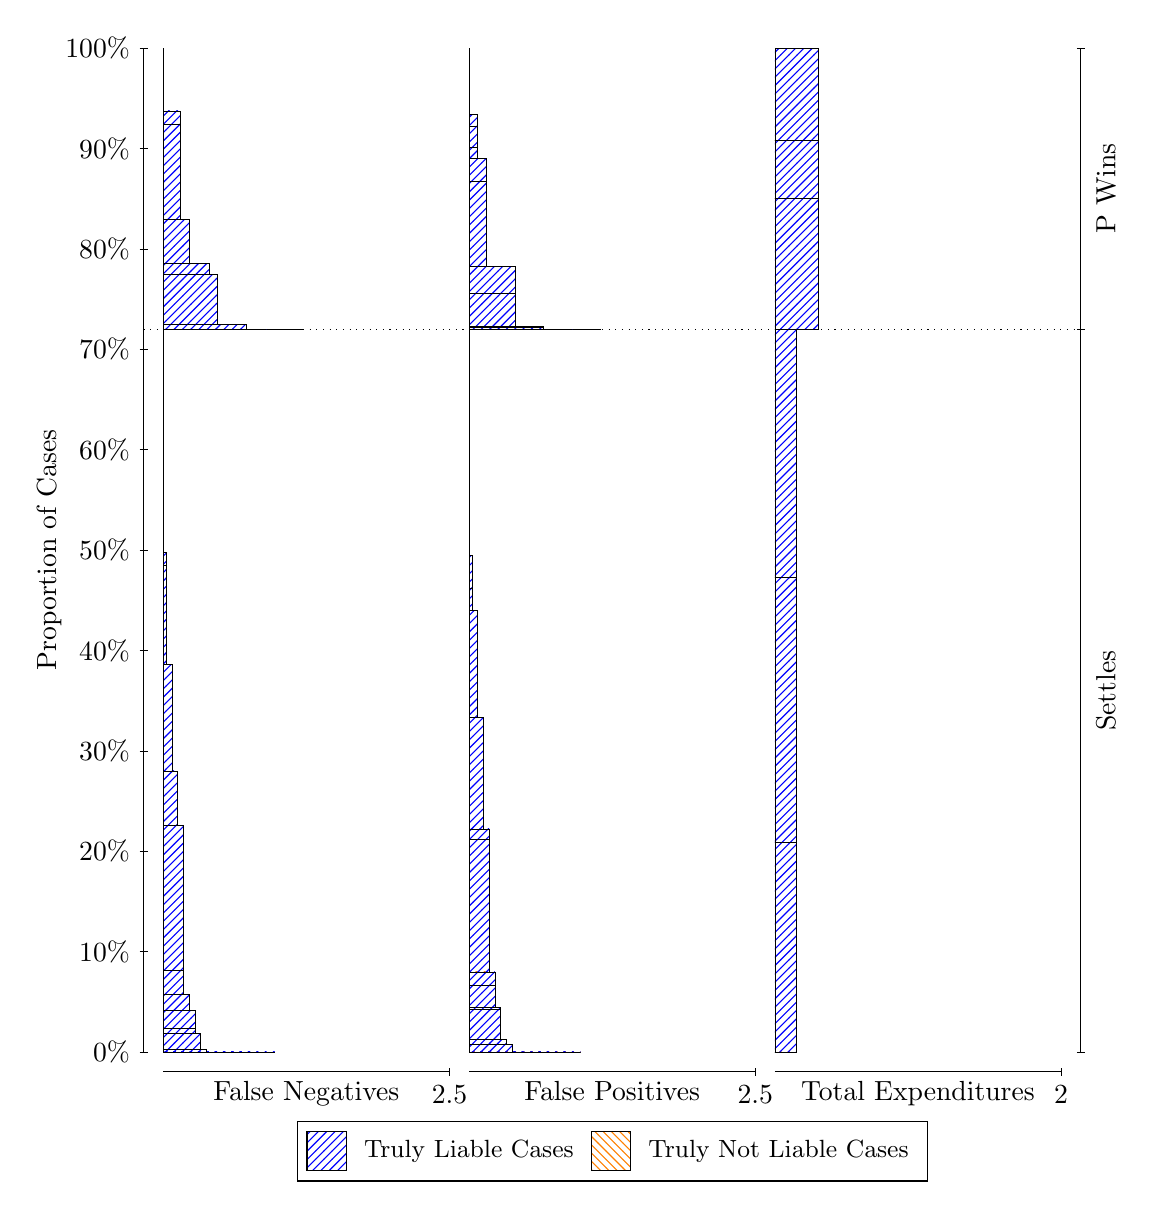
\begin{tikzpicture}
\draw[black, very thin] (1.5,1.75) -- (1.5,14.5);
\node[rotate=90, text=black, anchor=center] at (0.3, 8.125) {Proportion of Cases};
\draw[black, very thin] (1.45,1.75) -- (1.55,1.75);
\node[text=black, anchor=east] at (1.45, 1.75) {0\%};
\draw[black, very thin] (1.45,3.025) -- (1.55,3.025);
\node[text=black, anchor=east] at (1.45, 3.025) {10\%};
\draw[black, very thin] (1.45,4.3) -- (1.55,4.3);
\node[text=black, anchor=east] at (1.45, 4.3) {20\%};
\draw[black, very thin] (1.45,5.575) -- (1.55,5.575);
\node[text=black, anchor=east] at (1.45, 5.575) {30\%};
\draw[black, very thin] (1.45,6.85) -- (1.55,6.85);
\node[text=black, anchor=east] at (1.45, 6.85) {40\%};
\draw[black, very thin] (1.45,8.125) -- (1.55,8.125);
\node[text=black, anchor=east] at (1.45, 8.125) {50\%};
\draw[black, very thin] (1.45,9.4) -- (1.55,9.4);
\node[text=black, anchor=east] at (1.45, 9.4) {60\%};
\draw[black, very thin] (1.45,10.675) -- (1.55,10.675);
\node[text=black, anchor=east] at (1.45, 10.675) {70\%};
\draw[black, very thin] (1.45,11.95) -- (1.55,11.95);
\node[text=black, anchor=east] at (1.45, 11.95) {80\%};
\draw[black, very thin] (1.45,13.225) -- (1.55,13.225);
\node[text=black, anchor=east] at (1.45, 13.225) {90\%};
\draw[black, very thin] (1.45,14.5) -- (1.55,14.5);
\node[text=black, anchor=east] at (1.45, 14.5) {100\%};

\draw[black, very thin] (13.4,1.75) -- (13.4,14.5);
\draw[black, very thin] (13.35,1.75) -- (13.45,1.75);
\node[anchor=west] at (13.35, 1.75) {};
\draw[black, very thin] (13.35,10.928) -- (13.45,10.928);
\node[anchor=west] at (13.35, 10.928) {};
\draw[black, very thin] (13.35,14.5) -- (13.45,14.5);
\node[anchor=west] at (13.35, 14.5) {};

\draw[black, very thin, pattern color=blue, pattern=north east lines] (1.75,1.75) rectangle (3.167,1.75);
\draw[black, very thin, pattern color=blue, pattern=north east lines] (1.75,1.75) rectangle (3.0217,1.75);
\draw[black, very thin, pattern color=blue, pattern=north east lines] (1.75,1.75) rectangle (2.8763,1.75);
\draw[black, very thin, pattern color=blue, pattern=north east lines] (1.75,1.75) rectangle (2.8037,1.75);
\draw[black, very thin, pattern color=blue, pattern=north east lines] (1.75,1.75) rectangle (2.731,1.75);
\draw[black, very thin, pattern color=blue, pattern=north east lines] (1.75,1.75) rectangle (2.6583,1.75);
\draw[black, very thin, pattern color=blue, pattern=north east lines] (1.75,1.75) rectangle (2.5857,1.7504);
\draw[black, very thin, pattern color=blue, pattern=north east lines] (1.75,1.7504) rectangle (2.513,1.7504);
\draw[black, very thin, pattern color=blue, pattern=north east lines] (1.75,1.7504) rectangle (2.4403,1.7508);
\draw[black, very thin, pattern color=blue, pattern=north east lines] (1.75,1.7508) rectangle (2.3677,1.7508);
\draw[black, very thin, pattern color=blue, pattern=north east lines] (1.75,1.7508) rectangle (2.3677,1.7525);
\draw[black, very thin, pattern color=blue, pattern=north east lines] (1.75,1.7525) rectangle (2.295,1.7831);
\draw[black, very thin, pattern color=blue, pattern=north east lines] (1.75,1.7831) rectangle (2.2223,1.9849);
\draw[black, very thin, pattern color=blue, pattern=north east lines] (1.75,1.9849) rectangle (2.1497,2.0506);
\draw[black, very thin, pattern color=blue, pattern=north east lines] (1.75,2.0506) rectangle (2.1497,2.2827);
\draw[black, very thin, pattern color=blue, pattern=north east lines] (1.75,2.2827) rectangle (2.077,2.4838);
\draw[black, very thin, pattern color=blue, pattern=north east lines] (1.75,2.4838) rectangle (2.0043,2.4841);
\draw[black, very thin, pattern color=blue, pattern=north east lines] (1.75,2.4841) rectangle (2.0043,2.7895);
\draw[black, very thin, pattern color=blue, pattern=north east lines] (1.75,2.7895) rectangle (2.0043,4.6231);
\draw[black, very thin, pattern color=blue, pattern=north east lines] (1.75,4.6231) rectangle (1.9317,5.3185);
\draw[black, very thin, pattern color=blue, pattern=north east lines] (1.75,5.3185) rectangle (1.859,6.6755);
\draw[black, very thin, pattern color=blue, pattern=north east lines] (1.75,6.6755) rectangle (1.7863,7.9307);
\draw[black, very thin, pattern color=blue, pattern=north east lines] (1.75,7.9307) rectangle (1.7863,8.0955);
\draw[black, very thin, pattern color=orange, pattern=north west lines] (1.75,8.0955) rectangle (1.75,8.0955);
\draw[black, very thin, pattern color=blue, pattern=north east lines] (1.75,8.0955) rectangle (1.75,10.928);
\draw[black, very thin, pattern color=blue, pattern=north east lines] (1.75,10.928) rectangle (3.5303,10.928);
\draw[black, very thin, pattern color=blue, pattern=north east lines] (1.75,10.928) rectangle (3.167,10.929);
\draw[black, very thin, pattern color=blue, pattern=north east lines] (1.75,10.929) rectangle (3.058,10.929);
\draw[black, very thin, pattern color=blue, pattern=north east lines] (1.75,10.929) rectangle (2.8037,10.99);
\draw[black, very thin, pattern color=blue, pattern=north east lines] (1.75,10.99) rectangle (2.6947,10.99);
\draw[black, very thin, pattern color=blue, pattern=north east lines] (1.75,10.99) rectangle (2.4403,11.627);
\draw[black, very thin, pattern color=blue, pattern=north east lines] (1.75,11.627) rectangle (2.3313,11.767);
\draw[black, very thin, pattern color=blue, pattern=north east lines] (1.75,11.767) rectangle (2.077,12.326);
\draw[black, very thin, pattern color=blue, pattern=north east lines] (1.75,12.326) rectangle (1.968,13.53);
\draw[black, very thin, pattern color=blue, pattern=north east lines] (1.75,13.53) rectangle (1.968,13.701);
\draw[black, very thin, pattern color=orange, pattern=north west lines] (1.75,13.701) rectangle (1.75,13.701);
\draw[black, very thin, pattern color=blue, pattern=north east lines] (1.75,13.701) rectangle (1.75,14.5);
\draw[black, very thin, pattern color=orange, pattern=north west lines] (5.6333,1.75) rectangle (7.0503,1.75);
\draw[black, very thin, pattern color=blue, pattern=north east lines] (5.6333,1.75) rectangle (7.0503,1.75);
\draw[black, very thin, pattern color=orange, pattern=north west lines] (5.6333,1.75) rectangle (6.905,1.75);
\draw[black, very thin, pattern color=blue, pattern=north east lines] (5.6333,1.75) rectangle (6.905,1.75);
\draw[black, very thin, pattern color=orange, pattern=north west lines] (5.6333,1.75) rectangle (6.7597,1.75);
\draw[black, very thin, pattern color=blue, pattern=north east lines] (5.6333,1.75) rectangle (6.7597,1.75);
\draw[black, very thin, pattern color=blue, pattern=north east lines] (5.6333,1.75) rectangle (6.687,1.75);
\draw[black, very thin, pattern color=orange, pattern=north west lines] (5.6333,1.75) rectangle (6.6143,1.75);
\draw[black, very thin, pattern color=blue, pattern=north east lines] (5.6333,1.75) rectangle (6.6143,1.75);
\draw[black, very thin, pattern color=blue, pattern=north east lines] (5.6333,1.75) rectangle (6.5417,1.75);
\draw[black, very thin, pattern color=orange, pattern=north west lines] (5.6333,1.75) rectangle (6.469,1.75);
\draw[black, very thin, pattern color=blue, pattern=north east lines] (5.6333,1.75) rectangle (6.469,1.75);
\draw[black, very thin, pattern color=blue, pattern=north east lines] (5.6333,1.75) rectangle (6.3963,1.75);
\draw[black, very thin, pattern color=orange, pattern=north west lines] (5.6333,1.75) rectangle (6.3237,1.75);
\draw[black, very thin, pattern color=blue, pattern=north east lines] (5.6333,1.75) rectangle (6.3237,1.7508);
\draw[black, very thin, pattern color=orange, pattern=north west lines] (5.6333,1.7508) rectangle (6.3237,1.7508);
\draw[black, very thin, pattern color=blue, pattern=north east lines] (5.6333,1.7508) rectangle (6.3237,1.751);
\draw[black, very thin, pattern color=blue, pattern=north east lines] (5.6333,1.751) rectangle (6.251,1.7513);
\draw[black, very thin, pattern color=orange, pattern=north west lines] (5.6333,1.7513) rectangle (6.1783,1.7513);
\draw[black, very thin, pattern color=blue, pattern=north east lines] (5.6333,1.7513) rectangle (6.1783,1.8441);
\draw[black, very thin, pattern color=blue, pattern=north east lines] (5.6333,1.8441) rectangle (6.1057,1.9088);
\draw[black, very thin, pattern color=orange, pattern=north west lines] (5.6333,1.9088) rectangle (6.033,1.9088);
\draw[black, very thin, pattern color=blue, pattern=north east lines] (5.6333,1.9088) rectangle (6.033,2.2956);
\draw[black, very thin, pattern color=blue, pattern=north east lines] (5.6333,2.2956) rectangle (6.033,2.3169);
\draw[black, very thin, pattern color=blue, pattern=north east lines] (5.6333,2.3169) rectangle (5.9603,2.5927);
\draw[black, very thin, pattern color=blue, pattern=north east lines] (5.6333,2.5927) rectangle (5.9603,2.7661);
\draw[black, very thin, pattern color=orange, pattern=north west lines] (5.6333,2.7661) rectangle (5.8877,2.7661);
\draw[black, very thin, pattern color=blue, pattern=north east lines] (5.6333,2.7661) rectangle (5.8877,4.445);
\draw[black, very thin, pattern color=blue, pattern=north east lines] (5.6333,4.445) rectangle (5.8877,4.5825);
\draw[black, very thin, pattern color=blue, pattern=north east lines] (5.6333,4.5825) rectangle (5.815,6.0025);
\draw[black, very thin, pattern color=blue, pattern=north east lines] (5.6333,6.0025) rectangle (5.7423,7.3594);
\draw[black, very thin, pattern color=blue, pattern=north east lines] (5.6333,7.3594) rectangle (5.6697,7.634);
\draw[black, very thin, pattern color=blue, pattern=north east lines] (5.6333,7.634) rectangle (5.6697,8.0548);
\draw[black, very thin, pattern color=blue, pattern=north east lines] (5.6333,8.0548) rectangle (5.6333,10.928);
\draw[black, very thin, pattern color=orange, pattern=north west lines] (5.6333,10.928) rectangle (7.3047,10.928);
\draw[black, very thin, pattern color=blue, pattern=north east lines] (5.6333,10.928) rectangle (7.3047,10.928);
\draw[black, very thin, pattern color=orange, pattern=north west lines] (5.6333,10.928) rectangle (6.9413,10.928);
\draw[black, very thin, pattern color=blue, pattern=north east lines] (5.6333,10.928) rectangle (6.9413,10.928);
\draw[black, very thin, pattern color=blue, pattern=north east lines] (5.6333,10.928) rectangle (6.9413,10.928);
\draw[black, very thin, pattern color=orange, pattern=north west lines] (5.6333,10.928) rectangle (6.578,10.928);
\draw[black, very thin, pattern color=blue, pattern=north east lines] (5.6333,10.928) rectangle (6.578,10.954);
\draw[black, very thin, pattern color=blue, pattern=north east lines] (5.6333,10.954) rectangle (6.578,10.969);
\draw[black, very thin, pattern color=orange, pattern=north west lines] (5.6333,10.969) rectangle (6.469,10.969);
\draw[black, very thin, pattern color=blue, pattern=north east lines] (5.6333,10.969) rectangle (6.469,10.969);
\draw[black, very thin, pattern color=orange, pattern=north west lines] (5.6333,10.969) rectangle (6.2147,10.969);
\draw[black, very thin, pattern color=blue, pattern=north east lines] (5.6333,10.969) rectangle (6.2147,11.386);
\draw[black, very thin, pattern color=blue, pattern=north east lines] (5.6333,11.386) rectangle (6.2147,11.727);
\draw[black, very thin, pattern color=orange, pattern=north west lines] (5.6333,11.727) rectangle (6.1057,11.727);
\draw[black, very thin, pattern color=blue, pattern=north east lines] (5.6333,11.727) rectangle (6.1057,11.727);
\draw[black, very thin, pattern color=blue, pattern=north east lines] (5.6333,11.727) rectangle (6.1057,11.727);
\draw[black, very thin, pattern color=blue, pattern=north east lines] (5.6333,11.727) rectangle (5.8513,12.802);
\draw[black, very thin, pattern color=blue, pattern=north east lines] (5.6333,12.802) rectangle (5.8513,13.102);
\draw[black, very thin, pattern color=blue, pattern=north east lines] (5.6333,13.102) rectangle (5.7423,13.243);
\draw[black, very thin, pattern color=orange, pattern=north west lines] (5.6333,13.243) rectangle (5.7423,13.243);
\draw[black, very thin, pattern color=blue, pattern=north east lines] (5.6333,13.243) rectangle (5.7423,13.501);
\draw[black, very thin, pattern color=blue, pattern=north east lines] (5.6333,13.501) rectangle (5.7423,13.66);
\draw[black, very thin, pattern color=blue, pattern=north east lines] (5.6333,13.66) rectangle (5.6333,14.5);
\draw[black, very thin, pattern color=orange, pattern=north west lines] (9.5167,1.75) rectangle (9.7892,1.75);
\draw[black, very thin, pattern color=blue, pattern=north east lines] (9.5167,1.75) rectangle (9.7892,4.4096);
\draw[black, very thin, pattern color=orange, pattern=north west lines] (9.5167,4.4096) rectangle (9.7892,4.4096);
\draw[black, very thin, pattern color=blue, pattern=north east lines] (9.5167,4.4096) rectangle (9.7892,7.7757);
\draw[black, very thin, pattern color=orange, pattern=north west lines] (9.5167,7.7757) rectangle (9.7892,7.7757);
\draw[black, very thin, pattern color=blue, pattern=north east lines] (9.5167,7.7757) rectangle (9.7892,10.928);
\draw[black, very thin, pattern color=orange, pattern=north west lines] (9.5167,10.928) rectangle (10.062,10.928);
\draw[black, very thin, pattern color=blue, pattern=north east lines] (9.5167,10.928) rectangle (10.062,12.586);
\draw[black, very thin, pattern color=orange, pattern=north west lines] (9.5167,12.586) rectangle (10.062,12.586);
\draw[black, very thin, pattern color=blue, pattern=north east lines] (9.5167,12.586) rectangle (10.062,13.331);
\draw[black, very thin, pattern color=orange, pattern=north west lines] (9.5167,13.331) rectangle (10.062,13.331);
\draw[black, very thin, pattern color=blue, pattern=north east lines] (9.5167,13.331) rectangle (10.062,14.5);
\draw[black, dotted] (1.5,10.928) -- (13.4,10.928);
\draw[black, very thin] (1.75,1.5) -- (5.3833,1.5);
\node[text=black, anchor=north] at (3.5667, 1.5) {False Negatives};
\draw[black, very thin] (5.3833,1.45) -- (5.3833,1.55);
\node[text=black, anchor=north] at (5.3833, 1.45) {2.5};

\draw[black, very thin] (5.6333,1.5) -- (9.2667,1.5);
\node[text=black, anchor=north] at (7.45, 1.5) {False Positives};
\draw[black, very thin] (9.2667,1.45) -- (9.2667,1.55);
\node[text=black, anchor=north] at (9.2667, 1.45) {2.5};

\draw[black, very thin] (9.5167,1.5) -- (13.15,1.5);
\node[text=black, anchor=north] at (11.333, 1.5) {Total Expenditures};
\draw[black, very thin] (13.15,1.45) -- (13.15,1.55);
\node[text=black, anchor=north] at (13.15, 1.45) {2};

\node[text=black, centered, rotate=90] at (13.72, 6.339) {Settles};
\node[text=black, centered, rotate=90] at (13.72, 12.714) {P Wins};

\draw (7.449999999999999,1.5) node[draw=none] (baseCoordinate) {};
\begin{scope}[align=center]
        \matrix[scale=0.5, draw=black, below=0.5cm of baseCoordinate, nodes={draw}, column sep=0.1cm]{
            \node[rectangle, draw, minimum width=0.5cm, minimum height=0.5cm, pattern color=blue, pattern=north east lines] {}; &
            \node[draw=none, font=\small, text=black] (B) {Truly Liable Cases}; &
            \node[rectangle, draw, minimum width=0.5cm, minimum height=0.5cm, pattern color=orange, pattern=north west lines] {}; &
            \node[draw=none, font=\small, text=black] (B) {Truly Not Liable Cases}; \\
            };
\end{scope}

\end{tikzpicture}
\end{document}